\documentclass{article}
\usepackage[spanish]{babel}
\usepackage[utf8]{inputenc}
\usepackage{graphicx}
\usepackage{minted}

\title{\textbf{Criptografía aplicada: Cálculo del hash SHA-256 de un bloque Bitcoin}}
\author{Javier Domínguez Gómez \\
\small{jdg@member.fsf.org} \\
\small{Fingerprint: 94AD 19F4 9005 EEB2 3384 C20F 5BDC C668 D664 8E2B}}
\date{v0.1.03 - Febrero 2019}

\usepackage{courier}
\begin{document}
\maketitle

\tableofcontents{}

\section{Introducción}
    Este documento describe en detalle las partes de la cabecera de un bloque cualquiera en la cadena de bloques de Bitcoin, así como las operaciones lógico-matemáticas de la función criptográfica SHA-256 que se emplean con el fin de generar el \textit{hash} adecuado que finalmente representará dicho bloque en la cadena de bloques.

\section{Estructura de datos de un bloque}
    \vspace{3mm}
    Cada bloque de la cadena de bloques de Bitcoin contiene una estructura de datos que se puede categorizar en la siguiente tabla.
    \begin{table}[H]
    \centering
    \begin{tabular}{| c | l | c | l |} 
        \hline
        Tipo de dato & Nombre & Tamaño & Formato \\
        \hline
        uint32\_t & magicID & 4 bytes & Little-endian \\
        \hline
        uint32\_t & headerLenght & 4 bytes &  \\
        \hline
        uint32\_t & versionNumber & 4 bytes & Little-endian \\
        \hline
        uint8\_t[32] & previousBlockHash & 32 bytes & Big-endian \\
        \hline
        uint8\_t[32] & merkleRoot & 32 bytes & Big-endian \\
        \hline
        uint32\_t & timeStamp & 4 bytes & Little-endian \\
        \hline
        uint32\_t & targetDifficulty & 4 bytes & Little-endian \\
        \hline
        uint32\_t & nonce & 4 bytes & Little-endian \\
        \hline
        uint8/16/32/64\_t & transactionCount & 1, 3, 5 o 9 bytes &  \\
        \hline
    \end{tabular}
    \caption{\textit{Datos de la cabecera de un bloque en la cadena de bloques de Bitcoin.}}
    \label{table:0}
    \end{table}
    
    \subsection{magicID}
    Se trata de un dato de 4 bytes de longitud. Se establece como prefijo en cada uno de los mensajes entre los nodos para identificar la red de Bitcoin en la que se generan. La siguiente tabla muestra los diferentes valores que puede tener la variable magicID dependiendo de la red.
    
    \begin{table}[H]
    \centering
    \begin{tabular}{| c | c |} 
        \hline
        Red & magicID \\
        \hline
        Mainnet & \texttt{0xf9beb4d9} \\
        \hline
        Testnet & \texttt{0xfabfb5da} \\
        \hline
        Testnet3 & \texttt{0x0b110907} \\
        \hline
        Namecoin & \texttt{0xf9beb4fe} \\
        \hline
        Regtest & \texttt{0xfabfb5da} \\
        \hline
    \end{tabular}
    \label{table:1}
    \end{table}
    
    No solo sirve como dato identificativo de una red en particular, también cumple la función de delimitador entre mensajes y entre los datos de cada bloque, pues estos vienen concatenados en cadenas hexadecimales uno a continuación de otro.
    
    Se decidió establecer estos valores tan específicos dada la improbabilidad de que los caracteres ASCII que representan se encuentren en un mensaje estándar, tal y como se indica en el archivo \textit{chainparams.cpp}\footnote{https://github.com/bitcoin/bitcoin/blob/master/src/chainparams.cpp\#L99} que lo implementa en el código de Bitcoin.
    
    \subsection{headerLenght}
    \subsection{versionNumber}
    \subsection{previousBlockHash}
    \subsection{merkleRoot}
    \subsection{timeStamp}
    \subsection{targetDifficulty}
    \subsection{nonce}
    \subsection{transactionCount}
    En el caso de transactionCount el tipo de dato es un \textit{entero de longitud variable}\footnote{https://en.bitcoin.it/wiki/Protocol\_documentation\#Variable\_length\_integer}.
    
    \begin{figure}[H]
    \centering
        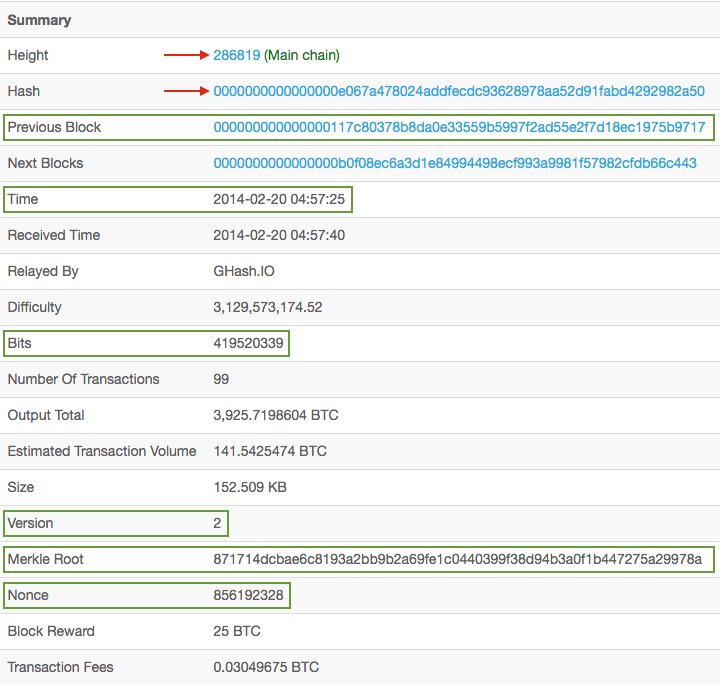
\includegraphics[scale=0.47]{img/Bitcoin_block_SHA_256_Block_Data}
        \caption{Datos empleados para la obtención del \textit{hash} del bloque $286819$.}
    \end{figure}
    
    \vspace{3mm}
    En la siguiente figura se detalla el contenido de los primeros 16 registros de la variable $W_{t}$ en cada una de las tres veces que se ejecutan las 64 iteraciones de la función SHA-256 para obtener el \textit{digest} en cada caso.
    \begin{figure}[H]
    \centering
        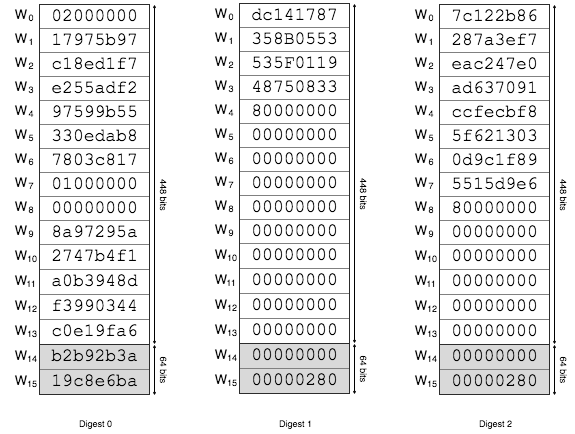
\includegraphics[scale=0.59]{img/Bitcoin_block_SHA_256_W0_W15_x3}
        \caption{Los primeros 16 registros de la variable $W_{t}$ en los tres casos en los que se ha de ejecutar la función SHA-256.}
    \end{figure}
\section{Fecha en formato Unix}
    \begin{figure}[H]
    \centering
        \begin{minted}{c}
    #include <stdio.h>
    #include <time.h>
    
    int main(int argc, char *argv[]) {
    
    	int year, month, day, hour, minute, second;
    	struct tm t;
    	time_t tod;
    
    	printf("Year: ");
    	scanf("%d", &year);
    	printf("Month: ");
    	scanf("%d", &month);
    	printf("Day: ");
    	scanf("%d", &day);
    	printf("Hour: ");
    	scanf("%d", &hour);
    	printf("Minute: ");
    	scanf("%d", &minute);
    	printf("Second: ");
    	scanf("%d", &second);
    
    	t.tm_year = year - 1900;
    	t.tm_mon = month - 1;   // Values [0-11]
    	t.tm_mday = day;
    	t.tm_hour = hour + 1;   // GMT+1
    	t.tm_min = minute;
    	t.tm_sec = second;
    	t.tm_isdst = 0;         // DST = 0
    	tod = mktime(&t);
    
    	printf("Timestamp epoch: %ld\n", (long) tod);
    }
        \end{minted}
    \end{figure}

\end{document}
